\section{Theorie}
\label{sec:Theorie}

\subsection{Fehlerrechnung}

Für die Fehlerfortpflanzung bei Gleichungen mit $N$ fehlerbehafteten Größen
wird jeweils die Formel zur Gaußschen Fehlerfortpflanzung

\begin{equation}
  \sigma = \sqrt{\sum_{i=1}^{N}\biggl(\frac{\partial f(x_i)}{\partial x_i}
  \sigma_i\biggr)^2}
\end{equation}
mit der jeweiligen Funktion $f(x_i)$, den Messgrößen $x_i$ und den
zugehörigen Fehlern $\sigma_i$ verwendet.
Zur Berechnung des arithmetischen Mittels von $N$ Messwerten wird jeweils die
Formel

\begin{equation}
  \bar{x} = \frac{1}{N}\sum_{i=1}^{N}x_i
\end{equation}
mit den Messwerten $x_i$ benutzt.
die Standardabweichung des Mittelwerts wird jeweils mit der Gleichung

\begin{equation}
  \bar{\sigma} = \sqrt{\frac{1}{N-1}\sum_{i=1}^{N}(x_i - \bar{x})^2}
\end{equation}
mit den $N$ Messwerten $x_i$ berechnet.

\subsection{Problemstellung}

Ein Körper an den Kräfte angreifen kann dadurch eine Volumenänderung oder eine
Verformung erfahren. Wenn die Kraft auf die Flächeneinheit bezogen wird, wird sie
als Spannung $\sigma$ bezeichnet. Der Zusammenhang zwischen der Volumenänderung
und der Spannung ist in vielen Fällen linear. Bezeichnet wird dieser Zusammenhang
als Hookesches Gesetz \eqref{eqn:hook}.

\begin{equation}
  \sigma = \symup{E} \frac{\Delta L}{L}
  \label{eqn:hook}
\end{equation}

Hier wird die Änderung in einer Dimension, der Längenänderung $L$, beschrieben;
dabei ist die Spannung eine Tangentialspannung. Eine schematische Darstellung ist
in Abbildung \ref{fig:dehnung} zu sehen.

\begin{figure}[h]
  \centering
  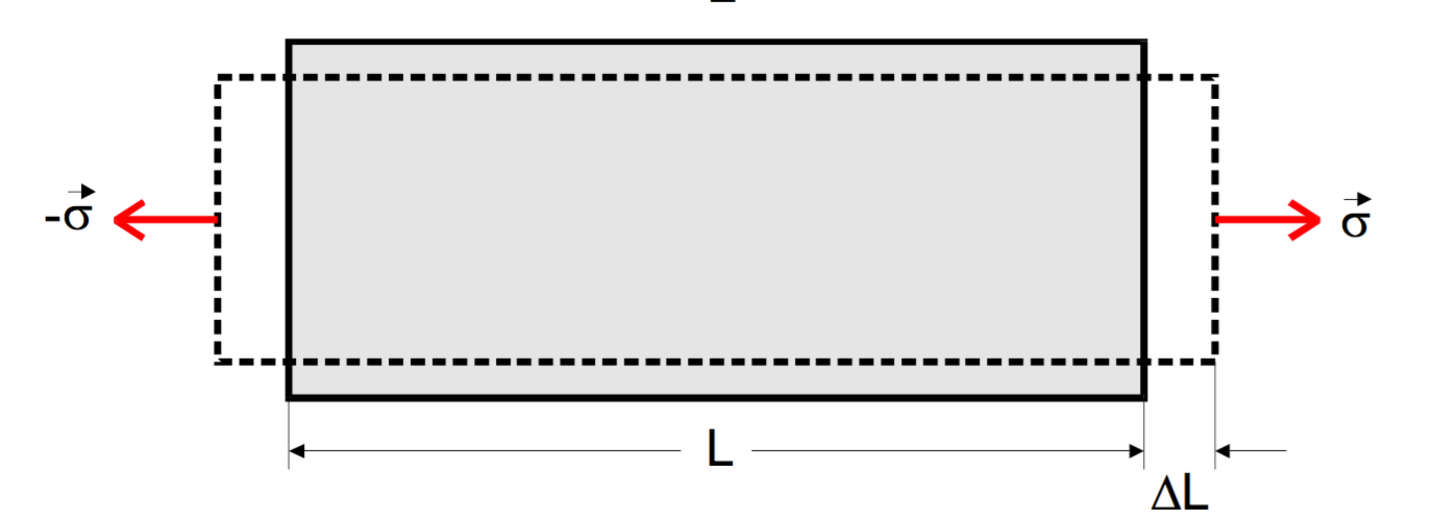
\includegraphics[width = \textwidth]{pics/dehnung.pdf}
  \caption{Längenänderung eines Stabes auf Grund einer Tangentialspannung\cite{anleitung}.}
  \label{fig:dehnung}
\end{figure}

Der Proportionalitätsfaktor $\symup{E}$ ist die in diesem Versuch zu bestimmende
Größe, der Elastizitätsmodul.
Da allerdings eine Längenänderung oft schwer zu messen ist, wird in diesem
Versuch $\symup{E}$ über die Biegung der zu untersuchenden Materialien bestimmt.
Dabei können mit relativ geringer Krafteinwirkung gute Ergebnisse erzielt werden.

\subsection{Biegung eines Stabes bei einseitiger Aufhängung}

Bei diesem Aufbau wird an den Stab, der an einer Seite eingespannt ist,
 ein Gewicht angehängt, wodurch er sich
biegt. Diese Biegung ist auch auf Dehnung zurüchzuführen; nur dass hier die
Dehnung auf der Länge des Stabes nicht gleichmäßig ist. Auf der Unterseite des
Stabes wird sogar negative Dehnung, also Stauchung, vorgefunden. Die Durchbiegung,
also die Verschiebung eines Punktes vor und nach Belastung, wird durch die
später bestimmte Funktion $D(x)$ beschrieben. Darin ist erneut der Elastizitätsmodul
enthalten.

\begin{figure}[h]
  \centering
  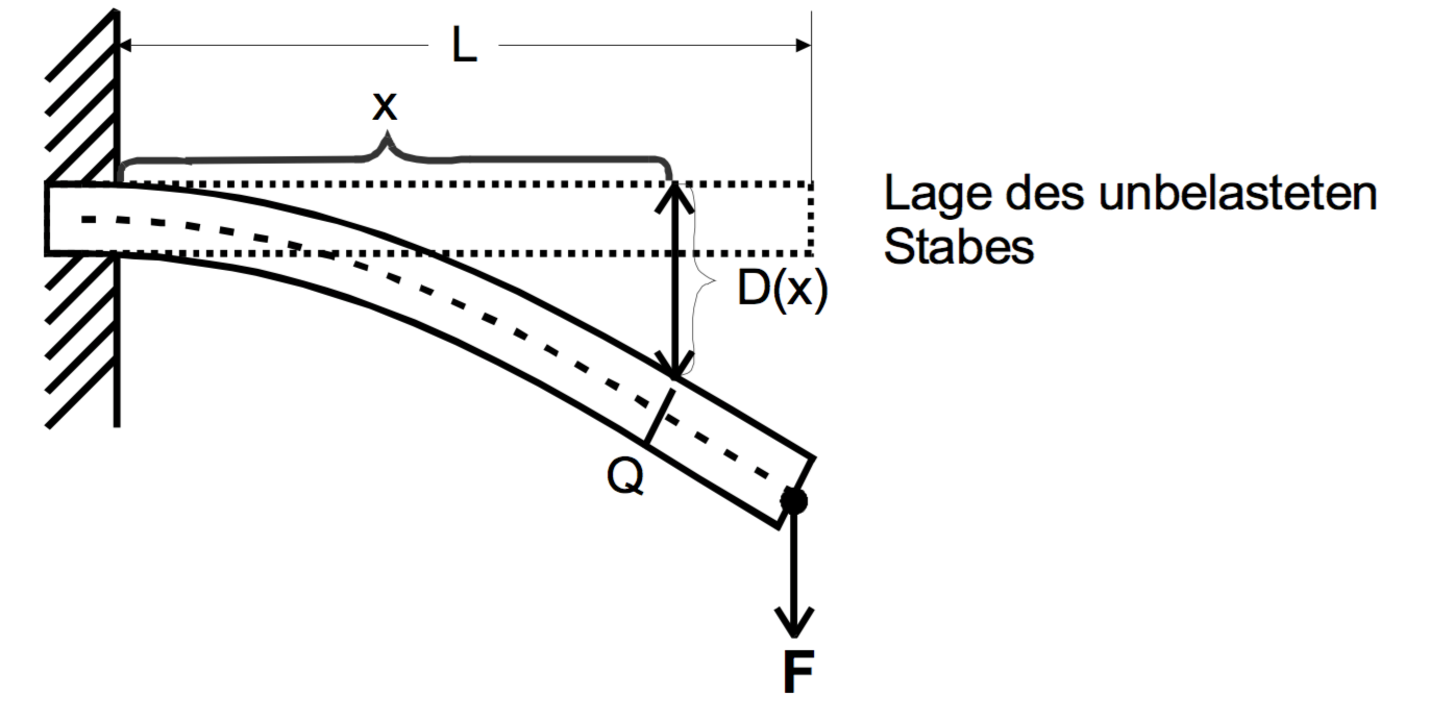
\includegraphics[width = \textwidth]{pics/biegungeinseit.pdf}
  \caption{Durchbiegung eines elastischen Stabes bei einseitiger Einspannung\cite{anleitung}.}
  \label{fig:biegungeinseit}
\end{figure}

In Abbildung \ref{fig:biegungeinseit} ist die Biegung nach $D(x)$ gegeben. Zu
erkennen ist auch die Querschnittsfläche $Q$, die aus ihrer vertikalen Position
verdreht ist. Dies geschieht auf Grund von Kräftepaaren, die entgegengesetzt
oben und unten an $Q$ angreifen. Dann müssen das Drehmoment betrachtet werden.

Wenn der Stab in Schichten aufgeteilt wird, haben die Oberen Zugspannung und die
Unteren Druckspannung. Die Schicht ohne jegliche Spannung, die auch die
ursprüngliche Länge beibehält, wird neutrale Faser genannt.

\begin{figure}[h]
  \centering
  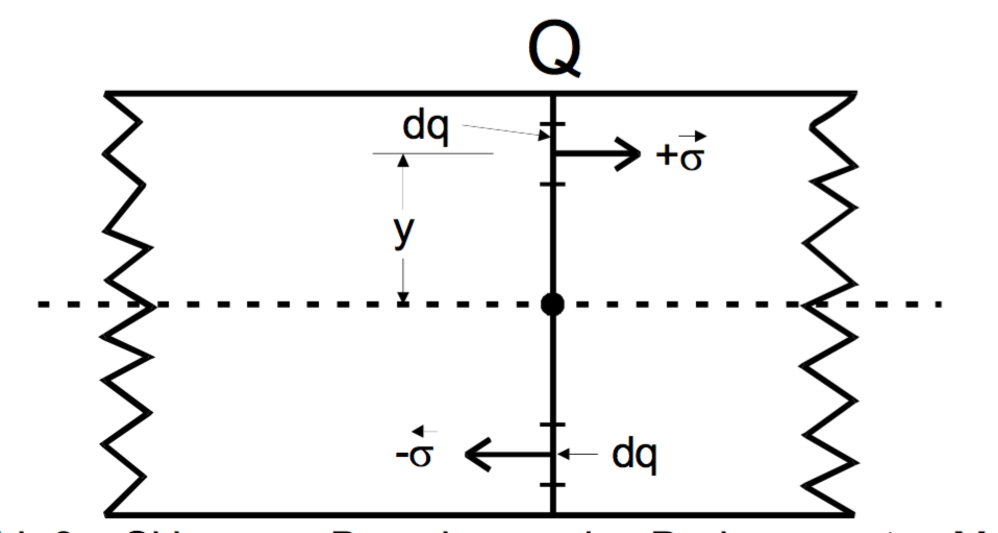
\includegraphics[height = 6cm]{pics/querschnittdreh.pdf}
  \caption{Skizze zur Berechnung des Drehmoments\cite{anleitung}.}
  \label{fig:querschnittdreh}
\end{figure}

Das Drehmoment $M_{\text{\sigma}}$ kann wie in Formel \eqref{eqn:drehmoment}
berechnet werden:

\begin{equation}
  M_{\text{\sigma}} = \int_{\text{Q}} y \sigma(y)\symup{d}q.
  \label{eqn:drehmoment}
\end{equation}

Dabei ist y der Abstand der Abstand zur neutralen Faser.
Über die Gleicheit der Drehmomente in Formel \eqref{eqn:mf=msigma}
wird die Momentengleichung \eqref{eqn:momenten} hergeleitet.

\begin{align}
  \intertext{mit}\\
  \g{M}_{\text{F}} = F (\g{L} - x)
  \label{eqn:aussenkraft}\\
  \symup{M}_{\text{F}} = \symup{M}_{\text{\sigma}}
  \label{eqn:mf=msigma}\\
  \symup{E}\frac{\g{d}^2 \g{D}}{\g{d}x^2} \underbrace{\int_{\g{Q}}y^2\g{d}q}_{\widehat{=} \g{I}}
   = F(\g{L} - x)
  \label{eqn:momenten}
\end{align}

Das markierte $\g{I}$ ist der Flächenträgheitsmoment. Nach Ausführen der
Integration ergibt sich für die Durchbiegung in Abhängigkeit von x, dem
Abstand zur Einspannung, Gleichung \eqref{eqn:durchbiegeinseit}.

\begin{equation}
  D(x) = \frac{F}{2 \g{E I}} \left( \g{L}x^2 - \frac{x^3}{3} \right)
  \label{eqn:durchbiegeinseit}
\end{equation}

\subsection{Biegung eines Stabes bei beidseitiger Auflage}

Bei diesem Aufbau wird der Stab an beiden Seiten aufgelegt und in der
Mitte des Stabs ein Gewicht angehängt.

\begin{figure}[h]
  \centering
  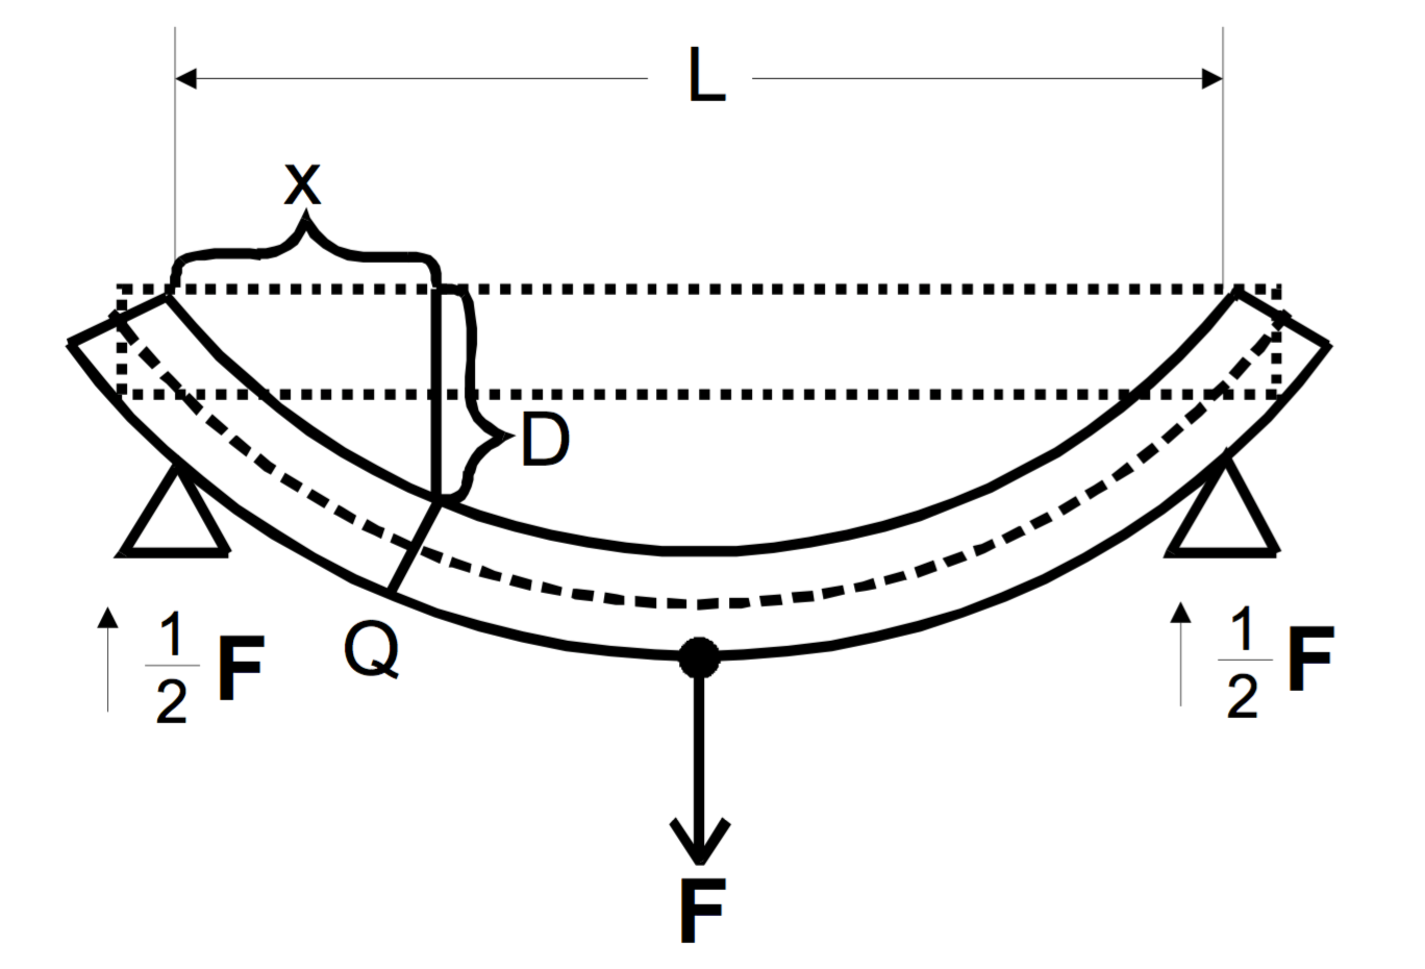
\includegraphics[height = 6cm]{pics/biegung2seit.pdf}
  \caption{Durchbiegung eines homogenen Stabes bei zweiseitiger Auflage\cite{anleitung}.}
  \label{fig:biegung2seit}
\end{figure}

Die Kräfteverteilung ist in Abbildung \ref{fig:biegung2seit} zu sehen.
Dann wird Gleichung \eqref{eqn:aussenkraft} zu Gleichung
\eqref{eqn:halbaussenkraft} mit einer Fallunterscheidung.

\begin{equation}\label{eqn:halbaussenkraft}
  \g{M}_{\text{F}} =
  \begin{cases}
     -\frac{F}{2} x, & 0 \leq x \leq \g{L}/2\\
     -\frac{F}{2} (\g{L} - x), & \g{L}/2 \leq x \leq \g{L}
  \end{cases}
\end{equation}

Die Momentengleichung \eqref{eqn:momentengleich2seit} sieht dann aus
wie folgt:

\begin{equation}
  \frac{\g{d}^2 D}{\g{d}x^2} = -\frac{F}{\g{E I}}\frac{x}{2} \text{ für }
  0 \leq x \leq \g{L}/2 \text{ bzw. } \frac{\g{d}^2 D}{\g{d}x^2} = -
  \frac{1}{2}\frac{F}{\g{E I}}(\g{L} - x) \text{ für } \g{L}/2 \leq x \leq \g{L}.
  \label{eqn:momentengleich2seit}
\end{equation}

Als Endergebnis ergibt sich dann Gleichung \eqref{eqn:durchbieg2seit1}
beziehungsweise Gleichung \eqref{eqn:durchbieg2seit2}.

\begin{align}
  D(x) &= \frac{F}{48\g{E I}} \left( 3\g{L}^2 x - 4 x^3 \right)
  &\text{ für } 0 \leq x \leq \g{L}/2
  \label{eqn:durchbieg2seit1}\\
  D(x) &= \frac{F}{48\g{E I}} \left( 4 x^3 - 12 \g{L}x^2 + 9\g{L}^2 x - \g{L}^3 \right)
  &\text{ für } \g{L}/2 \leq x \leq \g{L}
  \label{eqn:durchbieg2seit2}
\end{align}
